\documentclass{article}
\usepackage{tikz}
\usepackage{xcolor}

\definecolor{myblue}{RGB}{30,50,65}
\definecolor{bggray}{RGB}{240,240,240}

\begin{document}

\begin{center}
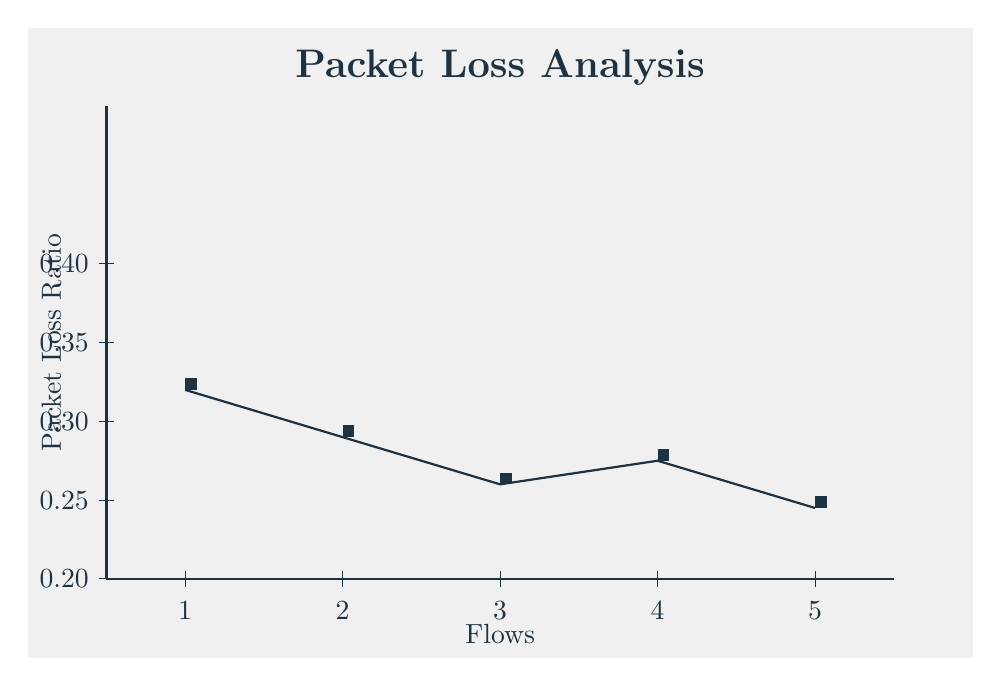
\begin{tikzpicture}

% Background
\fill[bggray] (0,0) rectangle (12,8);

% Axes
\draw[thick, myblue] (1,1) -- (1,7); % Y-axis
\draw[thick, myblue] (1,1) -- (11,1); % X-axis

% Title
\node[text=myblue, font=\Large\bfseries] at (6,7.5) {Packet Loss Analysis};

% Labels
\node[text=myblue] at (6,0.3) {Flows};
\node[rotate=90, text=myblue] at (0.3,4) {Packet Loss Ratio};

% Y-axis ticks (0.20–0.40)
\foreach \y/\val in {1/0.20,2/0.25,3/0.30,4/0.35,5/0.40} {
    \draw[myblue] (0.9,\y) -- (1.1,\y);
    \node[left, text=myblue] at (0.9,\y) {\val};
}

% X-axis ticks (1–5)
\foreach \x in {2,4,6,8,10} {
    \draw[myblue] (\x,0.9) -- (\x,1.1);
}
\node[text=myblue] at (2,0.6) {1};
\node[text=myblue] at (4,0.6) {2};
\node[text=myblue] at (6,0.6) {3};
\node[text=myblue] at (8,0.6) {4};
\node[text=myblue] at (10,0.6) {5};

% Scaling (0.20–0.40 → 1–7)
\def\scale{30}

% Data points
\coordinate (p1) at (2,{1 + (0.28-0.20)*\scale});
\coordinate (p2) at (4,{1 + (0.26-0.20)*\scale});
\coordinate (p3) at (6,{1 + (0.24-0.20)*\scale});
\coordinate (p4) at (8,{1 + (0.25-0.20)*\scale});
\coordinate (p5) at (10,{1 + (0.23-0.20)*\scale});

% Line
\draw[myblue, thick] (p1) -- (p2) -- (p3) -- (p4) -- (p5);

% Square markers
\foreach \p in {p1,p2,p3,p4,p5} {
    \fill[myblue] (\p) rectangle ++(0.15,0.15);
}

\end{tikzpicture}
\end{center}

\end{document}